% Apresentações em widescreen. Outros valores possíveis: 1610, 149, 54, 43 e 32.
% Por padrão, as apresentações são no formato 4:3 (sem o aspectratio).
\documentclass[aspectratio=43]{beamer}

\usetheme{Antibes}
\usecolortheme{default}
\usefonttheme[onlymath]{serif}			% para fontes matemáticas
% Enconte mais temas e cores em http://www.hartwork.org/beamer-theme-matrix/
% Veja também http://deic.uab.es/~iblanes/beamer_gallery/index.html

% Customizações de Cores: fg significa cor do texto e bg é cor do fundo
\setbeamercolor{normal text}{fg=black}
\setbeamercolor{alerted text}{fg=red}
\setbeamercolor{author}{fg=black}
\setbeamercolor{institute}{fg=blue}
\setbeamercolor{date}{fg=black}
\setbeamercolor{frametitle}{fg=white}
\setbeamercolor{framesubtitle}{fg=brown}
\setbeamercolor{block title}{bg=blue, fg=white}		%Cor do título
\setbeamercolor{block body}{bg=gray, fg=darkgray}	%Cor do texto (bg= fundo; fg=texto)

% ---
% PACOTES
% ---
\usepackage[alf]{abntex2cite}		% Citações padrão ABNT
\usepackage[brazil]{babel}		% Idioma do documento
\usepackage{color}			% Controle das cores
\usepackage[T1]{fontenc}		% Selecao de codigos de fonte.
\usepackage{graphicx}			% Inclusão de gráficos
\usepackage[utf8]{inputenc}		% Codificacao do documento (conversão automática dos acentos)
\usepackage{txfonts}			% Fontes virtuais
% ---

% --- Informações do documento ---
\title{Apresentação da documentação do sistema Solus}
\author{Angelo Silva}
\institute{Instituto Federal de Educação, Ciência e Tecnologia de São Paulo Câmpus Boituva
	    \par
	    Curso de Análise e Desenvolvimento de sistemas}
\date{\today, v-0.0.1}
% ---

% ----------------- INÍCIO DO DOCUMENTO --------------------------------------
\begin{document}

\frame{\titlepage}

% ----------------- NOVO SLIDE --------------------------------
\begin{frame}{Sumário}
\tableofcontents
\end{frame}

% ----------------- NOVO SLIDE --------------------------------
\begin{frame}{Construção}
\section{Construção}

A documentação do projeto foi construída utilizando lateX e o framework abnteX.

\vspace{0.1in}

O projeto pode ser encontrado em: \textbf{github.com/r6d6/solus}
\end{frame}

\begin{frame}{Introdução}
\section{Introdução}

Na sociedade contemporânea, diversas preocupações quanto a captação de energia surgiram. Uma dessas preocupações é cada vez mais, buscar fontes renováveis de energia.
\end{frame}

\begin{frame}{Descrição geral do sistema}
\section{Descrição geral do sistema}

O projeto visa, através da análise estatística de dados meteorológicos, auxiliar o estudo de viabilidade acerca da instalação de painéis fotovoltaicos.

Para isso, serão coletados dados através de sensores conectados a um microcontrolador arduino. Inicialmente, prevemos captar informações de umidade do ar, temperatura e incidência de radiação solar.
\end{frame}

\begin{frame}{Requisitos do sistema}
\section{Requisitos do sistema}

\begin{figure}[!htb]
    \label{figure_diagrama_caso_uso}
    \centering
    \caption{Diagrama de caso de uso} \label{includegraphics_diagrama_caso_uso}
    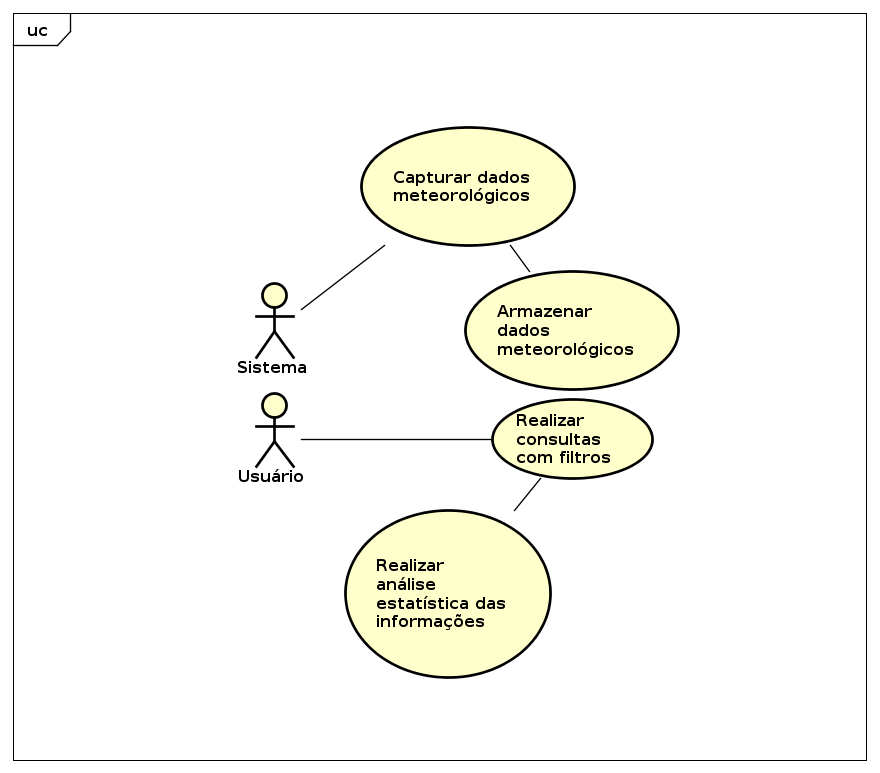
\includegraphics[scale=0.3]{caso_de_uso.png}
    \hfill
\end{figure}
\end{frame}

\begin{frame}{Tecnologias empregadas}
\section{Tecnologias empregadas}

\begin{itemize}
\item Microcontrolador arduino e suas libraries para requisição HTTP
\item GIT como sistema de versionamento para versionamento
\item PHP para criação da API
\item Lumen como framework para construção da API
\item Percona Server como SGBD (MySQL)
\item Docker para gerenciamento dos containers da aplicação \ldots
\end{itemize}
\end{frame}

\begin{frame}{Regras de negócio}
A maior parte das regras de negócio de sistema fica centralizada nos filtros, eles são quem validam os dados do sistema, definindo regras para a captura de dados.
A regra de negócio de filtragem diz que os dados de umidade e temperatura não podem se diferenciar por 50\% ou mais da média dos dados captados na ultima hora.
\end{frame}

% --- O comando \allowframebreaks ---
% Se o conteúdo não se encaixa em um quadro, a opção allowframebreaks instrui
% beamer para quebrá-lo automaticamente entre dois ou mais quadros,
% mantendo o frametitle do primeiro quadro (dado como argumento) e acrescentando
% um número romano ou algo parecido na continuação.

% \begin{frame}[allowframebreaks]{Referências}
% \bibliography{abntex2-modelo-references}
% \end{frame}

% ----------------- FIM DO DOCUMENTO -----------------------------------------
\end{document}
